\chapter{2015}
\section*{一、 选择题(本大题共 20 小题,每小题 2 分,共 40 分)}

1. 下面程序段的时间复杂度为(   )。

\begin{lstlisting}[language=C, basicstyle=\ttfamily]
m=10,n=10;s=0;
for (i=0;i<m;i++)
    for (j=0;j<n;j++)
        s+=i*j;
\end{lstlisting}

A. \(O\left( {m}^{2}\right)\) B. \(O\left( {n}^{2}\right)\)

C. \(O\left( {{m}^{ * }n}\right)\) D. \(O\left( 1\right)\)

2. 在线性表的下列运算中,不改变数据元素之间结构关系的运算是(   )。

A. 插入 B. 删除

C. 排序 D. 查找

3. 线性表采用链表存储时地址(   )。

A. 必须是连续的 B. 部分地址必须是连续的

C. 一定是不连续的 D. 连续不连续都可以

4. 在解决计算机主机与打印机之间速度不匹配问题时通常设置一个打印数据缓冲区,主机将要输出的数据依次写入该缓冲区,而打印机则依相同次序从该缓冲区中取出数据打

印。该缓冲区作为数据结构是一个(   )结构。

A. 栈 B. 队列 C. 哈希表 (Hash Table) D. 线性表

5. 一个栈的输入序列为 1, 2, 3, 4,下面哪一个序列不可能是这个栈的输出序列(   )？

A.2,3,4,1 B.4,3,1,2

C.1,3,2,4 D.3,4,2,1

6. 设计一个判别表达式中左、右括号是否配对出现的算法, 采用 (   ) 数据结构最佳。

A. 栈 B. 队列 C. 顺序结构线性表 D. 链式结构线性表

注:所有答案必须写在答题纸上,试卷上作答无效！

7. 在长度为 \(\mathrm{n}\) 顺序实现的线性表的第 \(\mathrm{i}\left( {1 \leq  \mathrm{i} \leq  \mathrm{n}}\right)\) 个位置之前插入一个元素,需要后移 (   )个元素。

A. 0 B. i C. 1 D. n-i+1 (10.3.15)

8. 链表不具有的特点是(   )。

A. 可随机访问任一元素 B. 插入、删除不需要移动元素

C. 不必事先估计存储空间 D. 所需空间与线性表长度成正比

9. 将一个 \(\mathrm{A}\left\lbrack  {20}\right\rbrack  \left\lbrack  {20}\right\rbrack\) (下标从 1 开始计算)的矩阵按行优先顺序存放,每个元素占 4 个存储单元,并且 \(\mathrm{A}\left\lbrack  1\right\rbrack  \left\lbrack  2\right\rbrack\) 的存储地址是 1004,则 \(\mathrm{A}\left\lbrack  {20}\right\rbrack  \left\lbrack  2\right\rbrack\) 的地址是(   )。

A. 1004 B. 1380 C. 1520 D. 2524

10. 树根的层数为 1 ,则一棵含 12 个结点的二叉树的高度至多为(   )。

A. 3 B. 4 C. 11 D. 12

11. 已知二叉树如下图,下列序列中,(   )是后序遍历后得到的序列。

\begin{center}
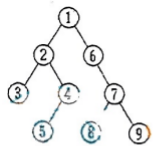
\includegraphics[width=0.2\textwidth]{images/2015/choice_11.png}
\hspace*{3em} 
\end{center}

\begin{tabular}{lccccccccc}
\text{A.3} & 5 & 4 & 2 & 8 & 9 & 7 & 6 & 1 \\
\text{B.3} & 4 & 5 & 2 & 8 & 9 & 7 & 6 & 1 \\
\text{C.1} & 2 & 3 & 4 & 5 & 6 & 7 & 8 & 9 \\
\text{D.2} & 3 & 4 & 5 & 6 & 7 & 8 & 9 & 1 \\
\end{tabular}

12. 已知数据表 A 中每个元素距其最终位置不远,则采用(   )排序算法最节省时间。

A. 堆排序 B. 直接插入排序 C. 快速排序 D. 简单选择排序

13. 请指出在顺序表 \(\{ 2\) 、5、7、10、14、15、18、23、35、41、 \({52}\}\) 中,用二分法查找关键码 12 需做多少次关键码比较(   )。

A. 2 B. 3 C. 5 D. 4

14. 查找 Hash 表,不会发生冲突的哈希函数是(   )。

A. 除留余数法 B. 伪随机探测再散列

C. 直接地址法 D. 线性探测再散列法

15. 对包含 N 个元素的散列表进行查找,平均查找长度(   )。

A、为 \(\mathrm{O}\left( {{\log }_{2}\mathrm{N}}\right)\) B、为 \(\mathrm{O}\left( \mathrm{N}\right)\) C、不直接依赖于 \(\mathrm{N}\) D、上述三者都不是

16. 下面四棵树中,数字表示相应叶子结点的权值,则(   )是哈夫曼树。 

A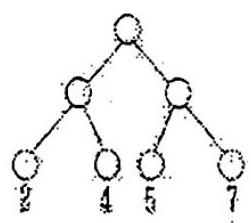
\includegraphics[width=0.2\textwidth]{images/2015/choice_16_A.jpg}
B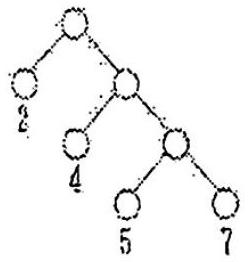
\includegraphics[width=0.2\textwidth]{images/2015/choice_16_B.jpg}
C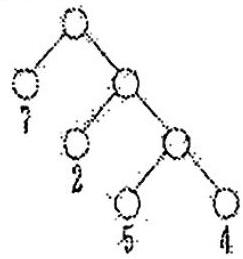
\includegraphics[width=0.2\textwidth]{images/2015/choice_16_C.jpg}
D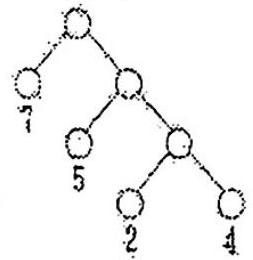
\includegraphics[width=0.2\textwidth]{images/2015/choice_16_D.jpg}

17. 下列排序算法中,(   )算法可能会出现下面情况:初始数据有序时,花费时间反而最多。 

A. 堆排序 B. 冒泡排序 C. 快速排序 D. 直接插入排序

18. 给定下列有向图和初始结点 V1,按深度优先遍历的结点序列为(   )。

\begin{center}
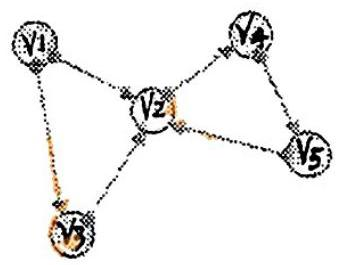
\includegraphics[width=0.2\textwidth]{images/2015/choice_18.jpg}
\end{center}
\hspace*{3em} 

A、V1, V3, V4, V5, V2

B、V1, V2, V3, V4, V5

C、V1, V2, V5, V3, V4

D、V1, V2, V4, V5, V3

19. 下面关于图的存储的叙述中, 哪一个是正确的(   )。

A. 用邻接矩阵法存储图,占用的存储空间数只与图中结点个数有关,而与边数无关。

B. 用邻接矩阵法存储图,占用的存储空间数只与图中边数有关,而与结点个数无关。

C. 用邻接表法存储图,占用的存储空间数只与图中结点个数有关,而与边数无关。

D. 用邻接表法存储图,占用的存储空间数只与图中边数有关,而与结点个数无关。

20. 在有向图的邻接表存储结构中,顶点 \(\mathrm{v}\) 在表结点中出现的次数等于(   )。

A. 顶点 \(\mathrm{v}\) 的度 B. 顶点 \(\mathrm{v}\) 的出度

C. 顶点 \(\mathrm{v}\) 的入度 D. 依附于顶点 \(\mathrm{v}\) 的边数

\section*{二、填空题(本大题共 17 小题,每小题 2 分,共 34 分)}

1. 设有一空队列 \(Q\) ,经 \(Q.{EnQueue}\left( 1\right) ,Q.{DeQueue}\left( \right) ,Q.{EnQueue}\left( 2\right) ,Q.{EnQueue}\left( 3\right) ,\) Q. EnQueue(4), Q. DeQueue (   ); Q. EnQueue (5)一系列操作后。队列中从队首到队尾的元素依次是\_\_\_\_\_。

2. 设栈 \(S\) 和队列 \(Q\) 的初始状态为空,元素 \(a\) 、 \(b\) 、 \(c\) 、 \(d\) 、 \(e\) 、 \(f\) 将依次入栈 \(S\) ,一个元素出栈后即进入队列 \(\mathrm{Q}\) 。若这 6 个元素出队列的顺序是 \(\mathrm{b}\text{ 、 }\mathrm{d}\text{ 、 }\mathrm{c}\text{ 、 }\mathrm{f}\text{ 、 }\mathrm{e}\text{ 、 }\mathrm{a}\) ,则栈 \(\mathrm{S}\) 的容量至少应该是\_\_\_\_\_,上述过程才不会错。

3. 已知完全二叉树的第 6 层(根结点为第 1 层)总共只有 5 个结点,则其叶子结点数是\_\_\_\_\_。

4. 用顺序存储的方法将完全二叉树中的所有结点逐层存放在数组 \(R\left\lbrack  {0,..,n - 1}\right\rbrack\) (下标从 0 开始计)中,结点 \(\mathrm{R}\left\lbrack  \mathrm{i}\right\rbrack\) 若有右子女,则右子女结点的下标是\_\_\_\_\_。

5. 某表达式二叉树按先序遍历的结果为 \(+ {\mathrm{a}}^{ * } + \mathrm{{bcd}}\) ,令 \(\mathrm{a} = 6,\mathrm{\;b} = 3,\mathrm{c} = 4,\mathrm{\;d} = 2\) ,则该表达式的值等于\_\_\_\_\_。

6. n 个元素的线性表,采用顺序存储结构,插入一个元素要平均移动表中\_\_\_\_\_个元素(假定在线性表任何位置上插入元素都是等概率的)。

7. 在一棵二叉树中, 度为 2 的结点有 50 个, 度为 1 的结点有 20 个, 该二叉树共有\_\_\_\_\_条边。

8. 含 12 个结点的平衡二叉树的最大深度是\_\_\_\_\_(设根节点的深度是 1)。

9. 设二叉树 \(\mathrm{T}\) 的前序遍历序列和中序遍历序列分别是: \(\mathrm{b},\mathrm{d},\mathrm{c},\mathrm{a},\mathrm{e},\mathrm{f}\) 和 \(\mathrm{c},\mathrm{d},\mathrm{e},\mathrm{a},\mathrm{b},\mathrm{f}\) ,则其后序遍历序列为\_\_\_\_\_。

10.6 阶 B-树 (B-Tree) 中, 每个结点至多包含 5 个关键码, 除根和叶结点外, 每个结点至少包含\_\_\_\_\_个关键码。

11. 具有 n 个叶子结点的哈夫曼树中,其结点总数为\_\_\_\_\_个。

12. G 为无向图,如果从 \(G\) 的某个顶点出发进行一次遍历,即可访问图的每个顶点,则该图一定是\_\_\_\_\_图。

13. 在一个图中,所有顶点的度数之和等于图的边数的\_\_\_\_\_倍。

14. 已知一个无向图的邻接矩阵表示,计算第 j 个结点的度的方法是\_\_\_\_\_。

15. 两个不同的关键字, 其哈希函数值相同, 因而被映射到同一表位置上, 这种现象称为\_\_\_\_\_。

\vspace{14em}

注:所有答案必须写在答题纸上,试卷上作答无效！ 第 5 页(共 9 页)

16. 对长度为 \(\mathrm{n}\) 的关键字序列进行快速排序的时间复杂度为\_\_\_\_\_。

17. 对于键值序列 \(\{ {12},{13},{11},{18},{60},{15},7,{18},{25},{100}\}\) 里建初始堆,必须从键值为\_\_\_\_\_的结点开始对每个结点进行一次堆调整。

\section*{三、问答题(本大题共 8 小题,每小题 7 分,共 56 分)}

1. 现有 2 棵树的森林如下图所示,请画出对应的二叉树。

\begin{center}
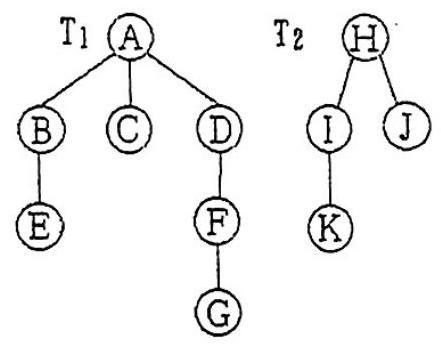
\includegraphics[width=0.3\textwidth]{images/2015/ask_1.jpg}
\end{center}
\hspace*{3em} 
\vspace{8em}

2. 已知关键字序列为36,31,20,32,66,48,依次将各元素插入到一棵初始为空的二叉排序树, 画出对应的二叉排序树。
\vspace{8em}

\newpage
3. 假设用于通信的电文由字符集 \(\{ \mathrm{A},\mathrm{B},\mathrm{C},\mathrm{D},\mathrm{E},\mathrm{F},\mathrm{G}\}\) 中的字母构成,这 7 个字母在电文中出现的频率依次为 \(\{ 3,{12},7,4,2,8,{11}\}\) 。请画出对应的编码哈夫曼树(Huffman)；求出每个字符的哈夫曼编码(约定编码时左分支编码 “0”,右分支编码为“1”。生成哈夫曼时, 同一层节点按左大右小排列)。
\vspace{8em}

4. 简要说明快速排序的排序思想。根据所给序列(49,38,65,97,76,13,27,50), 设选第一个元素为支点/参考值(pivot),写出快速排序的第一趟排序的结果。
\vspace{8em}

\newpage
5. 图 G 各顶点的连接关系及相应权值如下图所示。(1)画出该图的邻接距阵；(2)从顶点 V1 开始对图进行广度优先遍历,写出遍历结果(3)使用 Kruskal 算法求该图的最小生成树,画出其生成过程。

\begin{center}
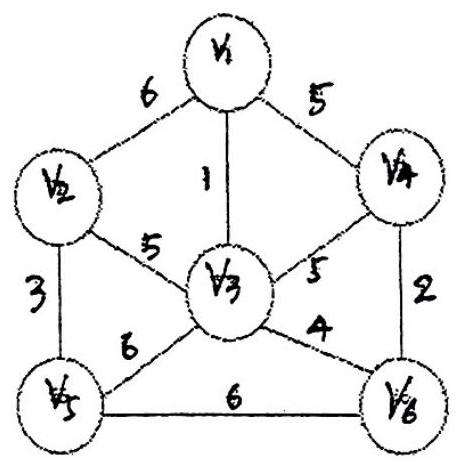
\includegraphics[width=0.3\textwidth]{images/2015/ask_5.jpg}
\end{center}
\hspace*{3em} 
\vspace{10em}

6. 以关键字序列(265,301,751,129,937,863,742,694,076,438)为例,分别写出执行以下排序算法的各趟排序状态和排序结束时关键字序列的状态。

(1)直接插入排序 

(2)希尔排序,增量序列为 5,3,1。上述方法中,哪些是稳定的排序？ 哪些是非稳定的排序?
\vspace{10em}

\newpage
7. 已知一组Key: (19 14 23 01 68 20 84 27 55 11 10 79), 按H(key) = key MOD 13 和 线性探测再散列 \(\mathrm{{Hi}} = \left( {\mathrm{H}\left( \mathrm{{key}}\right)  + \mathrm{{di}}}\right) \mathrm{{MOD}}\) 13 方法处理冲突,请画出最后得到的哈希表并填写相应的探测次数(完整下列表格即可)。

答: 哈希表如下:

\begin{center}
\begin{tabular}{|c|c|c|c|c|c|c|c|c|c|c|c|c|c|}
\hline
\phantom{X} & 0 & 1 & 2 & 3 & 4 & 5 & 6 & 7 & 8 & 9 & 10 & 11 & 12 \\
\cline{1-14}
哈希表 & \phantom{X} & \phantom{X} & \phantom{X} & \phantom{X} & \phantom{X} & \phantom{X} & \phantom{X} & \phantom{X} & \phantom{X} & \phantom{X} & \phantom{X} & \phantom{X} & \phantom{X} \\
\cline{1-14}
探测次数 & \phantom{X} & \phantom{X} & \phantom{X} & \phantom{X} & \phantom{X} & \phantom{X} & \phantom{X} & \phantom{X} & \phantom{X} & \phantom{X} & \phantom{X} & \phantom{X} & \phantom{X} \\
\cline{1-14}
\hline
\end{tabular}
\end{center}
\vspace{10em}

8. 利用 Dijkstra 算法求下图中从定点 \(\mathrm{V}1\) 到其他各定点间的最短路径,试用适杰斯特拉算法求出从顶点 \(\mathrm{a}\) 到其他各顶点间的最短路径,完成下表(最短路径用下划线标出):

\begin{center}
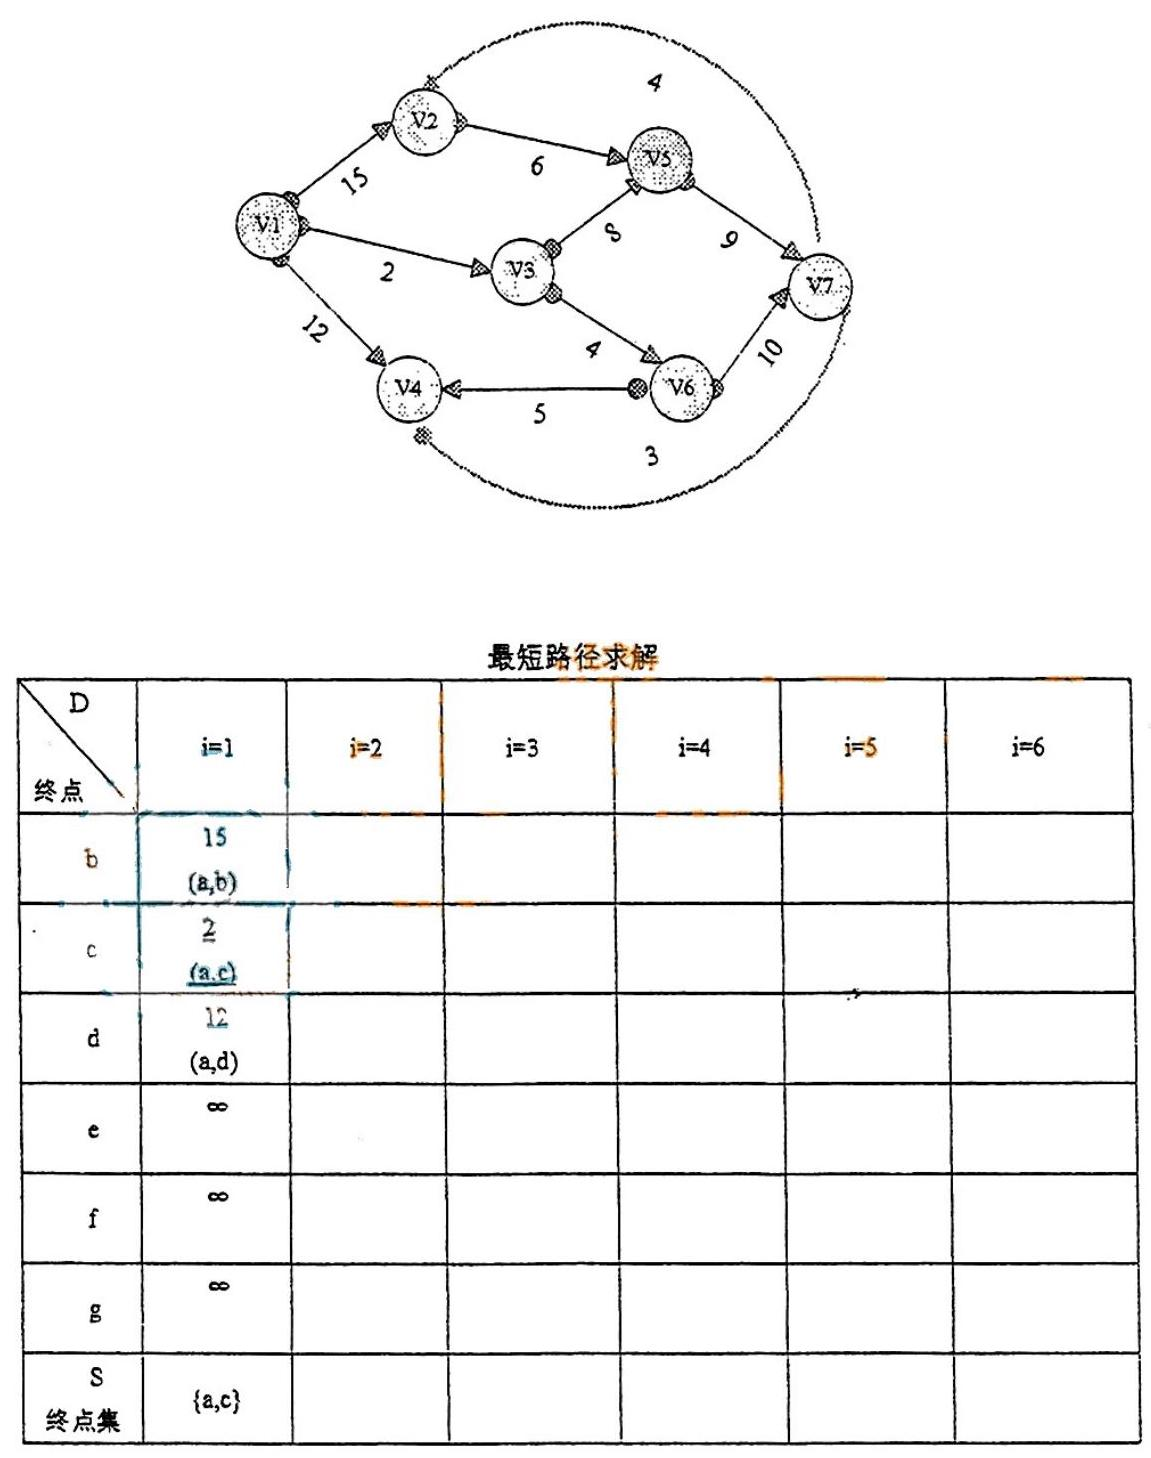
\includegraphics[width=0.9\textwidth]{images/2015/ask_8.jpg}
\end{center}
\vspace{15em}

\section*{四、算法设计、分析题(本大题共 2 小题,每小题 10 分,共 20 分)}

1. 设计一算法, 使得在尽可能少的时间内重排数组, 将所有取负值的关键字放在所有取非负值的关键字之前。

1)先给出算法思想；

2)再描述具体算法, 必要时请给予注释说明；

3)请分析算法的时间复杂度。
\vspace{15em}

2. 设计一算法判断某一二叉树是否为二叉排序树

1)二叉树用二叉链表的形式表示,定义如下:

typedef struct node\{

DataType data;

struct node *lchild,*rchild;

\}BinTNode;

2° 先给出算法思想,再描述算法,必要时请给予注释说明。
